% Options for packages loaded elsewhere
\PassOptionsToPackage{unicode}{hyperref}
\PassOptionsToPackage{hyphens}{url}
%
\documentclass[
]{article}
\usepackage{lmodern}
\usepackage{amssymb,amsmath}
\usepackage{ifxetex,ifluatex}
\ifnum 0\ifxetex 1\fi\ifluatex 1\fi=0 % if pdftex
  \usepackage[T1]{fontenc}
  \usepackage[utf8]{inputenc}
  \usepackage{textcomp} % provide euro and other symbols
\else % if luatex or xetex
  \usepackage{unicode-math}
  \defaultfontfeatures{Scale=MatchLowercase}
  \defaultfontfeatures[\rmfamily]{Ligatures=TeX,Scale=1}
\fi
% Use upquote if available, for straight quotes in verbatim environments
\IfFileExists{upquote.sty}{\usepackage{upquote}}{}
\IfFileExists{microtype.sty}{% use microtype if available
  \usepackage[]{microtype}
  \UseMicrotypeSet[protrusion]{basicmath} % disable protrusion for tt fonts
}{}
\makeatletter
\@ifundefined{KOMAClassName}{% if non-KOMA class
  \IfFileExists{parskip.sty}{%
    \usepackage{parskip}
  }{% else
    \setlength{\parindent}{0pt}
    \setlength{\parskip}{6pt plus 2pt minus 1pt}}
}{% if KOMA class
  \KOMAoptions{parskip=half}}
\makeatother
\usepackage{xcolor}
\IfFileExists{xurl.sty}{\usepackage{xurl}}{} % add URL line breaks if available
\IfFileExists{bookmark.sty}{\usepackage{bookmark}}{\usepackage{hyperref}}
\hypersetup{
  pdftitle={DS 621 Fall2020: Homework 3 (Group3)},
  pdfauthor={Zach Alexander, Sam Bellows, Donny Lofland, Joshua Registe, Neil Shah, Aaron Zalki},
  hidelinks,
  pdfcreator={LaTeX via pandoc}}
\urlstyle{same} % disable monospaced font for URLs
\usepackage[margin=1in]{geometry}
\usepackage{graphicx,grffile}
\makeatletter
\def\maxwidth{\ifdim\Gin@nat@width>\linewidth\linewidth\else\Gin@nat@width\fi}
\def\maxheight{\ifdim\Gin@nat@height>\textheight\textheight\else\Gin@nat@height\fi}
\makeatother
% Scale images if necessary, so that they will not overflow the page
% margins by default, and it is still possible to overwrite the defaults
% using explicit options in \includegraphics[width, height, ...]{}
\setkeys{Gin}{width=\maxwidth,height=\maxheight,keepaspectratio}
% Set default figure placement to htbp
\makeatletter
\def\fps@figure{htbp}
\makeatother
\setlength{\emergencystretch}{3em} % prevent overfull lines
\providecommand{\tightlist}{%
  \setlength{\itemsep}{0pt}\setlength{\parskip}{0pt}}
\setcounter{secnumdepth}{-\maxdimen} % remove section numbering
\usepackage{geometry}
\usepackage{multicol}
\usepackage{multirow}
\usepackage{xcolor}
\usepackage{booktabs}
\usepackage{longtable}
\usepackage{array}
\usepackage{wrapfig}
\usepackage{float}
\usepackage{colortbl}
\usepackage{pdflscape}
\usepackage{tabu}
\usepackage{threeparttable}
\usepackage{threeparttablex}
\usepackage[normalem]{ulem}
\usepackage{makecell}

\title{DS 621 Fall2020: Homework 3 (Group3)}
\usepackage{etoolbox}
\makeatletter
\providecommand{\subtitle}[1]{% add subtitle to \maketitle
  \apptocmd{\@title}{\par {\large #1 \par}}{}{}
}
\makeatother
\subtitle{Crime Logistic Regression}
\author{Zach Alexander, Sam Bellows, Donny Lofland, Joshua Registe, Neil Shah,
Aaron Zalki}
\date{}

\begin{document}
\maketitle

Source code:
\url{https://github.com/djlofland/DS621_F2020_Group3/tree/master/Homework_3}

\hypertarget{instructions}{%
\subsection{Instructions}\label{instructions}}

\hypertarget{overview}{%
\subsubsection{Overview}\label{overview}}

In this homework assignment, you will explore, analyze and model a data
set containing information on crime for various neighborhoods of a major
city. Each record has a response variable indicating whether or not the
crime rate is above the median crime rate (1) or not (0).

Your objective is to build a binary logistic regression model on the
training data set to predict whether the neighborhood will be at risk
for high crime levels. You will provide classifications and
probabilities for the evaluation data set using your binary logistic
regression model. You can only use the variables given to you (or
variables that you derive from the variables provided). Below is a short
description of the variables of interest in the data set:

\begin{itemize}
\tightlist
\item
  zn: proportion of residential land zoned for large lots (over 25000
  square feet) (predictor variable)
\item
  indus: proportion of non-retail business acres per suburb (predictor
  variable)
\item
  chas: a dummy var. for whether the suburb borders the Charles River
  (1) or not (0) (predictor variable)
\item
  nox: nitrogen oxides concentration (parts per 10 million) (predictor
  variable)
\item
  rm: average number of rooms per dwelling (predictor variable)
\item
  age: proportion of owner-occupied units built prior to 1940 (predictor
  variable)
\item
  dis: weighted mean of distances to five Boston employment centers
  (predictor variable)
\item
  rad: index of accessibility to radial highways (predictor variable)
\item
  tax: full-value property-tax rate per \$10,000 (predictor variable)
\item
  ptratio: pupil-teacher ratio by town (predictor variable)
\item
  lstat: lower status of the population (percent) (predictor variable)
\item
  medv: median value of owner-occupied homes in \$1000s (predictor
  variable)
\item
  target: whether the crime rate is above the median crime rate (1) or
  not (0) (response variable)
\end{itemize}

\hypertarget{deliverables}{%
\subsubsection{Deliverables}\label{deliverables}}

\begin{itemize}
\tightlist
\item
  A write-up submitted in PDF format. Your write-up should have four
  sections. Each one is described below. You may assume you are
  addressing me as a fellow data scientist, so do not need to shy away
  from technical details.
\item
  Assigned prediction (probabilities, classifications) for the
  evaluation data set. Use 0.5 threshold.
\item
  Include your R statistical programming code in an Appendix.
\end{itemize}

\hypertarget{introduction}{%
\subsection{Introduction}\label{introduction}}

Crime is a common concern in large cities, and denizens, policy makers
and law enforcement are interested in identifying locations where crime
can or might occur. In this assignment we are given a dataset for the
city of Boston, and will build a model to identify regions that might
have higher or lower (against the median) crime. Since the goal is a
binary (above or below median) response, this assignment will employ
binary logistic regression--and will not be predicting an actual value,
like the moneyball assignment.

\hypertarget{data-exploration}{%
\subsection{1. Data Exploration}\label{data-exploration}}

\emph{Describe the size and the variables in the crime training data
set. Consider that too much detail will cause a manager to lose interest
while too little detail will make the manager consider that you aren't
doing your job. Some suggestions are given below. Please do NOT treat
this as a check list of things to do to complete the assignment. You
should have your own thoughts on what to tell the boss. These are just
ideas.}

\hypertarget{dataset}{%
\subsubsection{Dataset}\label{dataset}}

The dataset is notably different from assignment 1's Moneyball
regression dataset in two ways: It contains both a categorical target,
and provides some categorical features. The fact that we are provided
with a categorical target turns the task from a regression task to a
classification task, perfect for logistic regression. The data contains
12 features and 466 instances, with 40 instances reserved for an
evaluation dataset with targets removed.

There are two files provided:

\begin{itemize}
\tightlist
\item
  \textbf{crime-training-data\_modified.csv} - hold data from training a
  model
\item
  \textbf{crime-evaluation-data\_modified.csv} - holdout data used to
  for evaluation. Note this dataset doesn't include the target column so
  while we can predict classes, our model will have to be scored by an
  outside group with knowledge of the actual classes.
\end{itemize}

Below, we created a chart that describes each variable in the dataset
and the theoretical effect it will have on the crime rate.

\begin{figure}
\centering
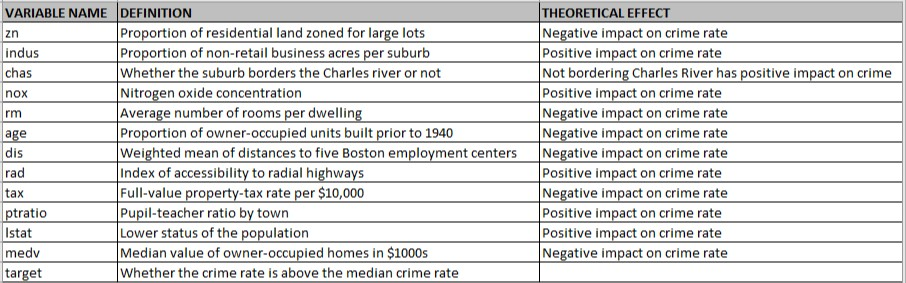
\includegraphics{./images/theoretical_effects.jpg}
\caption{Variables of Interest}
\end{figure}

\hypertarget{summary-stats}{%
\subsubsection{Summary Stats}\label{summary-stats}}

We compiled summary statistics on our dataset to better understand the
data before modeling.

\begin{verbatim}
##        zn             indus             chas              nox        
##  Min.   :  0.00   Min.   : 0.460   Min.   :0.00000   Min.   :0.3890  
##  1st Qu.:  0.00   1st Qu.: 5.145   1st Qu.:0.00000   1st Qu.:0.4480  
##  Median :  0.00   Median : 9.690   Median :0.00000   Median :0.5380  
##  Mean   : 11.58   Mean   :11.105   Mean   :0.07082   Mean   :0.5543  
##  3rd Qu.: 16.25   3rd Qu.:18.100   3rd Qu.:0.00000   3rd Qu.:0.6240  
##  Max.   :100.00   Max.   :27.740   Max.   :1.00000   Max.   :0.8710  
##        rm             age              dis              rad       
##  Min.   :3.863   Min.   :  2.90   Min.   : 1.130   Min.   : 1.00  
##  1st Qu.:5.887   1st Qu.: 43.88   1st Qu.: 2.101   1st Qu.: 4.00  
##  Median :6.210   Median : 77.15   Median : 3.191   Median : 5.00  
##  Mean   :6.291   Mean   : 68.37   Mean   : 3.796   Mean   : 9.53  
##  3rd Qu.:6.630   3rd Qu.: 94.10   3rd Qu.: 5.215   3rd Qu.:24.00  
##  Max.   :8.780   Max.   :100.00   Max.   :12.127   Max.   :24.00  
##       tax           ptratio         lstat             medv      
##  Min.   :187.0   Min.   :12.6   Min.   : 1.730   Min.   : 5.00  
##  1st Qu.:281.0   1st Qu.:16.9   1st Qu.: 7.043   1st Qu.:17.02  
##  Median :334.5   Median :18.9   Median :11.350   Median :21.20  
##  Mean   :409.5   Mean   :18.4   Mean   :12.631   Mean   :22.59  
##  3rd Qu.:666.0   3rd Qu.:20.2   3rd Qu.:16.930   3rd Qu.:25.00  
##  Max.   :711.0   Max.   :22.0   Max.   :37.970   Max.   :50.00  
##      target      
##  Min.   :0.0000  
##  1st Qu.:0.0000  
##  Median :0.0000  
##  Mean   :0.4914  
##  3rd Qu.:1.0000  
##  Max.   :1.0000
\end{verbatim}

The first observation is that we have no missing data (coded as NA's).

Based on the summary statistics, it appears we have some highly skewed
features, as many features have means that are far from the median
indicating a skewed distribution. Some examples include the variables
\texttt{zn} and \texttt{tax}. We also see a categorical variable
\texttt{chas} that appears to be quite imbalanced, as over 75\% of
values are 0.

\hypertarget{check-class-bias}{%
\subsubsection{Check Class Bias}\label{check-class-bias}}

We have two target values, 0 and 1. When building models, we ideally
want an equal representation of both classes. As class imbalance
deviates, our model performance will suffer both form effects of
differential variance between the classes and bias towards picking the
more represented class. For logistic regression, if we see strong
imbalance, we can 1) up-sample the smaller group, down-sample the larger
group, or adjust our threshold for assigning the predicted value away
from 0.5.

\begin{verbatim}
##    target 
## 0.4914163
\end{verbatim}

The classes are quite balanced, with approximately 51\% 0's and 49\%
1's. This is helpful, as with unbalanced class distributions it is often
necessary to artificially balance the classes to achieve good results.
No upsampling or downsampling will be required to achieve class balance
with this dataset.

\hypertarget{distributions}{%
\subsubsection{Distributions}\label{distributions}}

Next, we visualize the distribution profiles for each of the predictor
variables. This will help us to make a plan on which variable to
include, how they might be related to each other or the target, and
finally identify outliers or transformations that might help improve
model resolution.

\includegraphics{Homework3_Group3_files/figure-latex/unnamed-chunk-3-1.pdf}

The distribution profiles show the prevalence of kurtosis, specifically
right skew in variables \texttt{dis}, \texttt{lstat}, \texttt{nox},
\texttt{rm}, \texttt{zn}, and left skew in \texttt{age} and
\texttt{ptratio}. These deviations from a traditional normal
distribution can be problematic for linear regression assumptions, and
thus we might need to transform the data. The feature \texttt{chas} is
binary, as it only assumes values of 0 or 1. Furthermore, the features
\texttt{tax}, \texttt{rad}, and possibly \texttt{indus} appear bimodal.
Bimodal features in a dataset are both problematic and interesting and
potentially an area of opportunity and exploration. Bimodal data
suggests that there are possibly two different groups or classes within
the feature.

Bimodal features are extremely interesting in classification tasks, as
the could indicate overlapping but seperate distributions for each
class, which could provide powerful predictive power in a model.

While we don't tackle feature engineering in this analysis, if we were
performing a more in-depth analysis, we could leverage the package,
\texttt{mixtools} (see R Vignette). This package helps regress
\emph{mixed models} where data can be subdivided into subgroups.

Here is a quick example showing a possible mix within \texttt{indis}:

\begin{verbatim}
## number of iterations= 8
\end{verbatim}

\includegraphics{Homework3_Group3_files/figure-latex/unnamed-chunk-4-1.pdf}

Lastly, several features have both a distribution along with a high
number of values at an extreme. However, based on the feature meanings
and provided information, there is no reason to believe that any of
these extreme values are mistakes, data errors, or otherwise
inexplicable. As such, we will not remove the extreme values, as they
represent valuable data and could be predictive of the target.

\hypertarget{boxplots}{%
\subsubsection{Boxplots}\label{boxplots}}

In addition to creating histogram distributions, we also elected to use
box-plots to get an idea of the spread of each variable.

\includegraphics{Homework3_Group3_files/figure-latex/unnamed-chunk-5-1.pdf}

The box-plots reveal significant outliers that may need to be imputed if
necessary.

\hypertarget{variable-plots}{%
\subsubsection{Variable Plots}\label{variable-plots}}

Finally, we wanted to plot scatter plots of each variable versus the
target variable to get an idea of the relationship between them.

\includegraphics{Homework3_Group3_files/figure-latex/unnamed-chunk-6-1.pdf}

Although it does not appear that any 1 feature clearly distinguishes the
two target values, there are many features that appear to have some
significant correlation with the target, including \texttt{lstat},
\texttt{age}, \texttt{dis}, \texttt{zn}, and \texttt{nox}. This
indicates that our data may be predictive and the model building process
is likely to model an actual relationship rather than just overfitting
to the quirks of the training data.

\hypertarget{missing-data}{%
\subsubsection{Missing Data}\label{missing-data}}

Fortunately, we see no NAs, or missing data in the provided training
dataset.

\begin{verbatim}
##    values     ind
## 1       0      zn
## 2       0   indus
## 3       0    chas
## 4       0     nox
## 5       0      rm
## 6       0     age
## 7       0     dis
## 8       0     rad
## 9       0     tax
## 10      0 ptratio
## 11      0   lstat
## 12      0    medv
## 13      0  target
\end{verbatim}

\hypertarget{handle-outliers}{%
\subsubsection{Handle Outliers}\label{handle-outliers}}

As mentioned above, for this task we chose not to remove outliers as
there was no reason to believe that any of the values were in error.

\hypertarget{feature-target-correlations}{%
\subsubsection{Feature-Target
Correlations}\label{feature-target-correlations}}

With our outliers data imputed correctly, we can now build plots to
quantify the correlations between our target variable and predictor
variable. We will want to choose those with stronger positive or
negative correlations. Features with correlations closer to zero will
probably not provide any meaningful information on explaining crime
patterns.

\begin{verbatim}
##         values     ind
## 1   0.72610622     nox
## 2   0.63010625     age
## 3   0.62810492     rad
## 4   0.61111331     tax
## 5   0.60485074   indus
## 6   0.46912702   lstat
## 7   0.25084892 ptratio
## 8   0.08004187    chas
## 9  -0.15255334      rm
## 10 -0.27055071    medv
## 11 -0.43168176      zn
## 12 -0.61867312     dis
\end{verbatim}

It appears that \texttt{nox}, \texttt{age}, \texttt{rad}, \texttt{tax},
and \texttt{indus} have the highest correlation (positive) with
\texttt{target}; this appears to be somewhat counterintuitive, as older
buildings, more residential neighborhoods, and higher property tax
values appear to lead to higher crime, not what was expected. The strong
positive correlation with nitrous oxide is also interesting and
unexpected. The other variables have weak or slightly negative
correlation, which implies they have less predictive power.

\texttt{dis}, \texttt{zn}, and \texttt{medv} all have a negative
correlation to \texttt{target}, indicating that more distant areas with
large lot sizes and high median home values are less likely to be high
crime, all of which seems sensible.

\hypertarget{multicolinearity}{%
\subsubsection{Multicolinearity}\label{multicolinearity}}

One problem that can occur with multi-variable regression is correlation
between variables, or multicolinearity. A quick check is to run
correlations between variables.

\includegraphics{Homework3_Group3_files/figure-latex/unnamed-chunk-10-1.pdf}

We can see that some variables are highly correlated with one another,
such as \texttt{tax} and \texttt{rad}, with a correlation between .75
and 1. When we start considering features for our models, we'll need to
account for the correlations between features and avoid including pairs
with strong correlations.

As a note, this dataset is challenging as many of the predictive
features go hand-in-hand with other features and multicolinearity will
be a problem. Home size, price, age, and distance from employment
centers could all potentially be related, so it makes sense to see some
collinearity in the features.

\hypertarget{data-preparation}{%
\subsection{2. Data Preparation}\label{data-preparation}}

To summarize our data preparation and exploration, we can distinguish
our findings into a few categories below:

\hypertarget{removed-fields}{%
\subsubsection{Removed Fields}\label{removed-fields}}

All the predictor variables have no missing values and show no
indication of incomplete or incorrect data. As such, we have kept all
the fields.

\hypertarget{missing-values}{%
\subsubsection{Missing Values}\label{missing-values}}

The data had no missing values to remove.

\hypertarget{outliers}{%
\subsubsection{Outliers}\label{outliers}}

No outliers were removed as all values seemed reasonable.

\hypertarget{transform-non-normal-variables}{%
\subsubsection{Transform non-normal
variables}\label{transform-non-normal-variables}}

Finally, as mentioned earlier in our data exploration, and our findings
from our histogram plots, we can see that some of our variables are
highly skewed. To address this, we decided to perform some
transformations to make them more normally distributed. Here are some
plots to demonstrate the changes in distributions before and after the
transformations:

\includegraphics{Homework3_Group3_files/figure-latex/unnamed-chunk-11-1.pdf}
\includegraphics{Homework3_Group3_files/figure-latex/unnamed-chunk-11-2.pdf}

\hypertarget{finalizing-the-dataset-for-model-building}{%
\subsubsection{Finalizing the dataset for model
building}\label{finalizing-the-dataset-for-model-building}}

With our transformations complete, we can now add these into our
\texttt{clean\_df} dataframe and continue on to build our models.

\hypertarget{build-models}{%
\subsection{3. Build Models}\label{build-models}}

\emph{Using the training data, build at least three different binary
logistic regression models, using different variables (or the same
variables with different transformations). You may select the variables
manually, use an approach such as Forward or Stepwise, use a different
approach, or use a combination of techniques. Describe the techniques
you used. If you manually selected a variable for inclusion into the
model or exclusion into the model, indicate why this was done.} \emph{Be
sure to explain how you can make inferences from the model, as well as
discuss other relevant model output. Discuss the coefficients in the
models, do they make sense? Are you keeping the model even though it is
counter intuitive? Why? The boss needs to know.}

\hypertarget{model-building-methodology}{%
\subsubsection{Model-building
methodology}\label{model-building-methodology}}

With a solid understanding of our dataset at this point, and with our
data cleaned, we can now start to build out some of our binary logistic
regression models.

First, we decided to split our cleaned dataset into a training and
testing set (80\% training, 20\% testing). This was necessary as the
provided holdout evaluation dataset doesn't provide target values so we
cannot measure our model performance against that dataset.

First we decided to split our datasets (both original and transformed)
into test/train split (20/80).

Using our training dataset, we decided to run a binary logistic
regression model (Model \#1) that included all non-transformed features
that we hadn't removed following our data cleaning process mentioned
above.

\begin{verbatim}
## 
## Call:
## glm(formula = target ~ zn + indus + chas + nox + rm + age + dis + 
##     rad + tax + ptratio + lstat + medv, family = binomial, data = cleaneddftraining)
## 
## Deviance Residuals: 
##     Min       1Q   Median       3Q      Max  
## -1.8688  -0.2089  -0.0126   0.0058   3.2195  
## 
## Coefficients:
##               Estimate Std. Error z value Pr(>|z|)    
## (Intercept) -41.961957   7.618227  -5.508 3.63e-08 ***
## zn           -0.032397   0.032060  -1.011  0.31226    
## indus        -0.083574   0.053558  -1.560  0.11866    
## chas          1.602124   0.825019   1.942  0.05215 .  
## nox          47.057525   8.901809   5.286 1.25e-07 ***
## rm           -0.026319   0.857628  -0.031  0.97552    
## age           0.026183   0.014668   1.785  0.07425 .  
## dis           0.694392   0.242381   2.865  0.00417 ** 
## rad           0.452735   0.167328   2.706  0.00682 ** 
## tax          -0.004252   0.003210  -1.325  0.18532    
## ptratio       0.368844   0.147560   2.500  0.01243 *  
## lstat         0.118421   0.064655   1.832  0.06702 .  
## medv          0.158597   0.076652   2.069  0.03854 *  
## ---
## Signif. codes:  0 '***' 0.001 '**' 0.01 '*' 0.05 '.' 0.1 ' ' 1
## 
## (Dispersion parameter for binomial family taken to be 1)
## 
##     Null deviance: 516.31  on 372  degrees of freedom
## Residual deviance: 151.07  on 360  degrees of freedom
## AIC: 177.07
## 
## Number of Fisher Scoring iterations: 9
\end{verbatim}

We also calculated VIF scores to measure effects of collinearity:

\begin{verbatim}
## [1] "VIF scores of predictors"
\end{verbatim}

\begin{verbatim}
##       zn    indus     chas      nox       rm      age      dis      rad 
## 1.689851 2.720384 1.270717 4.311227 7.871620 2.508018 3.795841 1.792675 
##      tax  ptratio    lstat     medv 
## 2.151334 2.123881 3.140594 9.601022
\end{verbatim}

Model 2 was built using our transformed features.

\begin{verbatim}
## 
## Call:
## glm(formula = target ~ zn_transform + indus + chas + nox_transform + 
##     rm_transform + age_transform + dis_transform + rad + tax + 
##     ptratio_transform + lstat_transform + medv, family = binomial, 
##     data = cleaneddftraining)
## 
## Deviance Residuals: 
##     Min       1Q   Median       3Q      Max  
## -2.1914  -0.1960  -0.0149   0.0124   3.2134  
## 
## Coefficients:
##                    Estimate Std. Error z value Pr(>|z|)    
## (Intercept)       13.190685   8.345687   1.581  0.11398    
## zn_transform      -0.066517   0.243382  -0.273  0.78462    
## indus             -0.026601   0.054347  -0.489  0.62451    
## chas               1.347185   0.841578   1.601  0.10942    
## nox_transform     12.755697   2.318373   5.502 3.75e-08 ***
## rm_transform      -3.750350   3.103419  -1.208  0.22687    
## age_transform     -0.951540   0.309005  -3.079  0.00207 ** 
## dis_transform      3.418917   1.043777   3.276  0.00105 ** 
## rad                0.529029   0.190519   2.777  0.00549 ** 
## tax               -0.003521   0.003388  -1.040  0.29856    
## ptratio_transform -1.859276   0.619783  -3.000  0.00270 ** 
## lstat_transform    0.499170   0.833033   0.599  0.54903    
## medv               0.231388   0.076548   3.023  0.00250 ** 
## ---
## Signif. codes:  0 '***' 0.001 '**' 0.01 '*' 0.05 '.' 0.1 ' ' 1
## 
## (Dispersion parameter for binomial family taken to be 1)
## 
##     Null deviance: 516.31  on 372  degrees of freedom
## Residual deviance: 143.38  on 360  degrees of freedom
## AIC: 169.38
## 
## Number of Fisher Scoring iterations: 9
\end{verbatim}

We also calculated VIF scores to measure effects of collinearity:

\begin{verbatim}
## [1] "VIF scores of predictors"
\end{verbatim}

\begin{verbatim}
##      zn_transform             indus              chas     nox_transform 
##          1.539558          2.602237          1.246935          3.639147 
##      rm_transform     age_transform     dis_transform               rad 
##          6.542191          2.212741          4.007969          1.919888 
##               tax ptratio_transform   lstat_transform              medv 
##          2.274082          2.069956          4.294371          8.723338
\end{verbatim}

Our next model we used a Stepwise AIC on model 1 (our model with
non-transformed features) to pick which features were most relevant.

\begin{verbatim}
## 
## Call:
## glm(formula = target ~ indus + chas + nox + age + dis + rad + 
##     tax + ptratio + lstat + medv, family = binomial, data = cleaneddftraining)
## 
## Deviance Residuals: 
##      Min        1Q    Median        3Q       Max  
## -1.96754  -0.23736  -0.02428   0.00521   3.07687  
## 
## Coefficients:
##               Estimate Std. Error z value Pr(>|z|)    
## (Intercept) -42.777875   7.404584  -5.777 7.59e-09 ***
## indus        -0.089400   0.053898  -1.659 0.097182 .  
## chas          1.716995   0.797961   2.152 0.031419 *  
## nox          48.015921   9.043213   5.310 1.10e-07 ***
## age           0.026011   0.012244   2.124 0.033634 *  
## dis           0.582605   0.201400   2.893 0.003819 ** 
## rad           0.456431   0.156227   2.922 0.003483 ** 
## tax          -0.004810   0.003092  -1.555 0.119863    
## ptratio       0.409269   0.131868   3.104 0.001912 ** 
## lstat         0.121364   0.057970   2.094 0.036299 *  
## medv          0.153254   0.045197   3.391 0.000697 ***
## ---
## Signif. codes:  0 '***' 0.001 '**' 0.01 '*' 0.05 '.' 0.1 ' ' 1
## 
## (Dispersion parameter for binomial family taken to be 1)
## 
##     Null deviance: 516.31  on 372  degrees of freedom
## Residual deviance: 152.39  on 362  degrees of freedom
## AIC: 174.39
## 
## Number of Fisher Scoring iterations: 9
\end{verbatim}

We also calculated VIF scores to measure effects of collinearity:

\begin{verbatim}
## [1] "VIF scores of predictors"
\end{verbatim}

\begin{verbatim}
##    indus     chas      nox      age      dis      rad      tax  ptratio 
## 2.769481 1.226824 4.594466 1.801884 3.004437 1.653794 1.986334 1.657318 
##    lstat     medv 
## 2.537234 3.463469
\end{verbatim}

In our final model we used a Stepwise AIC on model 2 (our model with
transformed features) to pick which features were most relevant.

\begin{verbatim}
## 
## Call:
## glm(formula = target ~ chas + nox_transform + rm_transform + 
##     age_transform + dis_transform + rad + ptratio_transform + 
##     medv, family = binomial, data = cleaneddftraining)
## 
## Deviance Residuals: 
##     Min       1Q   Median       3Q      Max  
## -2.1434  -0.2423  -0.0233   0.0160   3.2134  
## 
## Coefficients:
##                   Estimate Std. Error z value Pr(>|z|)    
## (Intercept)       14.45154    5.83826   2.475 0.013312 *  
## chas               1.48267    0.79702   1.860 0.062847 .  
## nox_transform     12.56999    2.19920   5.716 1.09e-08 ***
## rm_transform      -4.56831    2.81334  -1.624 0.104418    
## age_transform     -0.91861    0.29048  -3.162 0.001565 ** 
## dis_transform      3.74400    0.93841   3.990 6.61e-05 ***
## rad                0.45409    0.15088   3.010 0.002616 ** 
## ptratio_transform -1.91150    0.57656  -3.315 0.000915 ***
## medv               0.24095    0.07322   3.291 0.000999 ***
## ---
## Signif. codes:  0 '***' 0.001 '**' 0.01 '*' 0.05 '.' 0.1 ' ' 1
## 
## (Dispersion parameter for binomial family taken to be 1)
## 
##     Null deviance: 516.31  on 372  degrees of freedom
## Residual deviance: 145.96  on 364  degrees of freedom
## AIC: 163.96
## 
## Number of Fisher Scoring iterations: 9
\end{verbatim}

We also calculated VIF scores to measure effects of collinearity:

\begin{verbatim}
## [1] "VIF scores of predictors"
\end{verbatim}

\begin{verbatim}
##              chas     nox_transform      rm_transform     age_transform 
##          1.160759          3.723046          5.780850          2.044138 
##     dis_transform               rad ptratio_transform              medv 
##          3.514481          1.269320          1.845819          8.496893
\end{verbatim}

\hypertarget{examining-our-model-coefficients}{%
\subsubsection{Examining our model
coefficients}\label{examining-our-model-coefficients}}

Throughout our model-building process, we noticed that many of our model
outputs yielded a few coefficient values that seemed to contradict our
initial estimates. For instance, in Model \#1:

\textbf{Positive values for coefficients that we'd expect to be
negative}

\begin{itemize}
\tightlist
\item
  age - logically we thought that the higher the proportion of
  owner-occupied units built prior to 1940 would lead to a lower crime
  rate (historic homes with more property value)
\item
  dis - logically we thought that the higher the weighted mean value of
  distance to five Boston employment centers, the lower the crime rate
  (areas farther from employment centers indicated there is less of a
  need for them -- higher rates of employment)
\item
  medv - logically we thought the higher the median value of
  owner-occupied homes in \$1000s would lead to a lower crime rate
\end{itemize}

This is a trend we saw throughout the four models that we built,
although Models \#3 and \#4 were able to adjust for this better than our
first two models -- we can likely attribute this phenomenon to
multicolinearity. Since we noticed in our initial data exploration that
many variables in the dataset were highly correlated with one another
(i.e.~\texttt{medv} and \texttt{zn}, \texttt{nox} and \texttt{indus},
\texttt{tax} and \texttt{rad}), this phenomenon likely is increasing the
variance of the coefficient estimates, making them difficult to
interpret (and in some cases such as the features listed above, they are
switching the signs). This was also supported by our Variance Inflation
Factor (VIF) tests, which showed high values for features such as
{[}\texttt{medv} and \texttt{rn}{]}. In our final models (Models \#3 and
\#4), we made sure to keep this in mind in order to get a better handle
on our coefficients and reduce multicolinearity -- mainly, we removed
certain variables that had high VIF scores through our stepwise
selection process.

\hypertarget{model-selection-analysis}{%
\subsection{4. Model Selection \&
Analysis}\label{model-selection-analysis}}

\emph{For the binary logistic regression model, will you use a metric
such as log likelihood, AIC, ROC curve, etc.? Using the training data
set, evaluate the binary logistic regression model based on (a)
accuracy, (b) classification error rate, (c) precision, (d) sensitivity,
(e) specificity, (f) F1 score, (g) AUC, and (h) confusion matrix. Make
predictions using the evaluation data set.}

Model \#1 Confusion Matrix

\begin{verbatim}
## Confusion Matrix and Statistics
## 
##           Reference
## Prediction  0  1
##          0 40 13
##          1  2 38
##                                          
##                Accuracy : 0.8387         
##                  95% CI : (0.748, 0.9068)
##     No Information Rate : 0.5484         
##     P-Value [Acc > NIR] : 2.979e-09      
##                                          
##                   Kappa : 0.6817         
##                                          
##  Mcnemar's Test P-Value : 0.009823       
##                                          
##             Sensitivity : 0.7451         
##             Specificity : 0.9524         
##          Pos Pred Value : 0.9500         
##          Neg Pred Value : 0.7547         
##              Prevalence : 0.5484         
##          Detection Rate : 0.4086         
##    Detection Prevalence : 0.4301         
##       Balanced Accuracy : 0.8487         
##                                          
##        'Positive' Class : 1              
## 
\end{verbatim}

Model \#2 Confusion Matrix

\begin{verbatim}
## Confusion Matrix and Statistics
## 
##           Reference
## Prediction  0  1
##          0 40  8
##          1  2 43
##                                           
##                Accuracy : 0.8925          
##                  95% CI : (0.8111, 0.9472)
##     No Information Rate : 0.5484          
##     P-Value [Acc > NIR] : 7.341e-13       
##                                           
##                   Kappa : 0.7856          
##                                           
##  Mcnemar's Test P-Value : 0.1138          
##                                           
##             Sensitivity : 0.8431          
##             Specificity : 0.9524          
##          Pos Pred Value : 0.9556          
##          Neg Pred Value : 0.8333          
##              Prevalence : 0.5484          
##          Detection Rate : 0.4624          
##    Detection Prevalence : 0.4839          
##       Balanced Accuracy : 0.8978          
##                                           
##        'Positive' Class : 1               
## 
\end{verbatim}

Model \#3 Confusion Matrix

\begin{verbatim}
## Confusion Matrix and Statistics
## 
##           Reference
## Prediction  0  1
##          0 40 13
##          1  2 38
##                                          
##                Accuracy : 0.8387         
##                  95% CI : (0.748, 0.9068)
##     No Information Rate : 0.5484         
##     P-Value [Acc > NIR] : 2.979e-09      
##                                          
##                   Kappa : 0.6817         
##                                          
##  Mcnemar's Test P-Value : 0.009823       
##                                          
##             Sensitivity : 0.7451         
##             Specificity : 0.9524         
##          Pos Pred Value : 0.9500         
##          Neg Pred Value : 0.7547         
##              Prevalence : 0.5484         
##          Detection Rate : 0.4086         
##    Detection Prevalence : 0.4301         
##       Balanced Accuracy : 0.8487         
##                                          
##        'Positive' Class : 1              
## 
\end{verbatim}

Model \#4 Confusion Matrix

\begin{verbatim}
## Confusion Matrix and Statistics
## 
##           Reference
## Prediction  0  1
##          0 39  8
##          1  3 43
##                                           
##                Accuracy : 0.8817          
##                  95% CI : (0.7982, 0.9395)
##     No Information Rate : 0.5484          
##     P-Value [Acc > NIR] : 4.648e-12       
##                                           
##                   Kappa : 0.7637          
##                                           
##  Mcnemar's Test P-Value : 0.2278          
##                                           
##             Sensitivity : 0.8431          
##             Specificity : 0.9286          
##          Pos Pred Value : 0.9348          
##          Neg Pred Value : 0.8298          
##              Prevalence : 0.5484          
##          Detection Rate : 0.4624          
##    Detection Prevalence : 0.4946          
##       Balanced Accuracy : 0.8859          
##                                           
##        'Positive' Class : 1               
## 
\end{verbatim}

A Comparison of ROC Curves

\includegraphics{Homework3_Group3_files/figure-latex/unnamed-chunk-26-1.pdf}

\begin{verbatim}
## 
## Call:
## roc.default(response = cleaneddftesting[["target"]], predictor = cleaneddftesting[["model1"]],     plot = TRUE, legacy.axes = TRUE, print.auc = TRUE)
## 
## Data: cleaneddftesting[["model1"]] in 42 controls (cleaneddftesting[["target"]] 0) < 51 cases (cleaneddftesting[["target"]] 1).
## Area under the curve: 0.8487
\end{verbatim}

\includegraphics{Homework3_Group3_files/figure-latex/unnamed-chunk-26-2.pdf}

\begin{verbatim}
## 
## Call:
## roc.default(response = cleaneddftesting[["target"]], predictor = cleaneddftesting[["model2"]],     plot = TRUE, legacy.axes = TRUE, print.auc = TRUE)
## 
## Data: cleaneddftesting[["model2"]] in 42 controls (cleaneddftesting[["target"]] 0) < 51 cases (cleaneddftesting[["target"]] 1).
## Area under the curve: 0.8978
\end{verbatim}

\includegraphics{Homework3_Group3_files/figure-latex/unnamed-chunk-26-3.pdf}

\begin{verbatim}
## 
## Call:
## roc.default(response = cleaneddftesting[["target"]], predictor = cleaneddftesting[["model3"]],     plot = TRUE, legacy.axes = TRUE, print.auc = TRUE)
## 
## Data: cleaneddftesting[["model3"]] in 42 controls (cleaneddftesting[["target"]] 0) < 51 cases (cleaneddftesting[["target"]] 1).
## Area under the curve: 0.8487
\end{verbatim}

\includegraphics{Homework3_Group3_files/figure-latex/unnamed-chunk-26-4.pdf}

\begin{verbatim}
## 
## Call:
## roc.default(response = cleaneddftesting[["target"]], predictor = cleaneddftesting[["model4"]],     plot = TRUE, legacy.axes = TRUE, print.auc = TRUE)
## 
## Data: cleaneddftesting[["model4"]] in 42 controls (cleaneddftesting[["target"]] 0) < 51 cases (cleaneddftesting[["target"]] 1).
## Area under the curve: 0.8859
\end{verbatim}

The following table discusses each of the model performance metrics on
the training dataset. These values indicate there is a minor improvement
in model performance after applying transformations and selecting for
significant parameters.

\begin{table}[H]
\centering
\begin{tabular}{l|r|r|r|r|r}
\hline
Model & Accuracy & F1 & Deviance & R2 & AIC\\
\hline
Model \#1 & 0.8487395 & 0.8351648 & 151.0663 & 0.7074132 & 177.0663\\
\hline
Model \#2 & 0.8977591 & 0.8958333 & 143.3803 & 0.7222995 & 169.3803\\
\hline
Model \#3 & 0.8487395 & 0.8351648 & 152.3886 & 0.7048521 & 174.3886\\
\hline
Model \#4 & 0.8858543 & 0.8865979 & 145.9614 & 0.7173004 & 163.9614\\
\hline
\end{tabular}
\end{table}

\hypertarget{todo-explain-the-results-of-model-outputs}{%
\subsection{TODO -- explain the results of model
outputs}\label{todo-explain-the-results-of-model-outputs}}

The analysis shows the following results:

Model 1 - This model is based on the all non-transformed variables.
Results for this model provided an F1 value of 0.94, but .

Model 2 - This model is based on a subset of significant predictors on
an un-transformed dataset. Results for this model provided an R\^{}2 of
about of 0.31 on the training set and 0.31 on the testing dataset.

Model 3 - This model is based on a subset of significant predictors on
an transformed dataset. Results for this model provided an R\^{}2 of
about of 0.31 on the training set and 0.31 on the testing dataset.

\hypertarget{todo-model-of-choice}{%
\subsection{TODO -- Model of choice}\label{todo-model-of-choice}}

Based on these analyses, Model 2 and Model 3 both performed marginally
better than Model 1 and could be selected as the linear model of choice
when looking at adjusted R2. However, there is greater statistical
significance under the third model relative to the others and uses less
unnecessary variables to compute our prediction without sacrificing much
in terms of adjusted R\^{}2 value. Additionally, Model 3 seems to have
lower VIF scores than Models 1 and 2. Because of these factors, as well
as its better adjustment for multicollinearity (we noticeably saw less
sign-flipping in coefficients), model 3 would be the model of choice.

\hypertarget{references}{%
\subsection{References}\label{references}}

\begin{itemize}
\tightlist
\item
  A Modern Approach to Regression with R: Simon Sheather
\item
  Linear Models with R: Julian Faraway.
\item
  R package vignette,
  \href{https://cran.r-project.org/web/packages/mixtools/vignettes/mixtools.pdf}{mixtools:
  An R Package for Analyzing Finite Mixture Models}
\item
  \href{https://statisticsbyjim.com/regression/ols-linear-regression-assumptions/}{7
  Classic OLS assumptions}
\item
  \href{https://online.stat.psu.edu/stat462/node/180/}{Detecting
  Multicolinearity with VIF}
\end{itemize}

\hypertarget{appendix}{%
\subsection{Appendix}\label{appendix}}

\hypertarget{a.-crime-dataset-columns}{%
\subsubsection{A. Crime Dataset
Columns}\label{a.-crime-dataset-columns}}

\begin{itemize}
\tightlist
\item
  \href{https://github.com/djlofland/DS621_F2020_Group3/tree/master/Homework_3}{Group
  3 HW 3 GitHub}
\end{itemize}

\hypertarget{r-code}{%
\subsubsection{R Code}\label{r-code}}

\begin{verbatim}
# =====================================================================================
# Load Libraries and Define Helper functions 
# =====================================================================================

library(MASS)
library(rpart.plot)
library(ggplot2)
library(ggfortify)
library(gridExtra)
library(forecast)
library(fpp2)
library(fma)
library(kableExtra)
library(e1071)
library(mlbench)
library(ggcorrplot)
library(DataExplorer)
library(timeDate)
library(caret)
library(GGally)
library(corrplot)
library(RColorBrewer)
library(tibble)
library(tidyr)
library(tidyverse)
library(dplyr)
library(reshape2)
library(mixtools)
library(tidymodels)
library(ggpmisc)
library(regclass)

#' Print a side-by-side Histogram and QQPlot of Residuals
#'
#' @param model A model
#' @examples
#' residPlot(myModel)
#' @return null
#' @export
residPlot <- function(model) {
  # Make sure a model was passed
  if (is.null(model)) {
    return
  }
  
  layout(matrix(c(1,1,2,3), 2, 2, byrow = TRUE))
  plot(residuals(model))
  hist(model[["residuals"]], freq = FALSE, breaks = "fd", main = "Residual Histogram",
       xlab = "Residuals",col="lightgreen")
  lines(density(model[["residuals"]], kernel = "ep"),col="blue", lwd=3)
  curve(dnorm(x,mean=mean(model[["residuals"]]), sd=sd(model[["residuals"]])), col="red", lwd=3, lty="dotted", add=T)
  qqnorm(model[["residuals"]], main = "Residual Q-Q plot")
  qqline(model[["residuals"]],col="red", lwd=3, lty="dotted")
  par(mfrow = c(1, 1))
}

#' Print a Variable Importance Plot for the provided model
#'
#' @param model The model
#' @param chart_title The Title to show on the plot
#' @examples
#' variableImportancePlot(myLinearModel, 'My Title)
#' @return null
#' @export
variableImportancePlot <- function(model=NULL, chart_title='Variable Importance Plot') {
  # Make sure a model was passed
  if (is.null(model)) {
    return
  }
  
  # use caret and gglot to print a variable importance plot
  varImp(model) %>% as.data.frame() %>% 
    ggplot(aes(x = reorder(rownames(.), desc(Overall)), y = Overall)) +
    geom_col(aes(fill = Overall)) +
    theme(panel.background = element_blank(),
          panel.grid = element_blank(),
          axis.text.x = element_text(angle = 90)) +
    scale_fill_gradient() +
    labs(title = chart_title,
         x = "Parameter",
         y = "Relative Importance")
}


#' Print a Facet Chart of histograms
#'
#' @param df Dataset
#' @param box Facet size (rows)
#' @examples
#' histbox(my_df, 3)
#' @return null
#' @export
histbox <- function(df, box) {
    par(mfrow = box)
    ndf <- dimnames(df)[[2]]
    
    for (i in seq_along(ndf)) {
            data <- na.omit(unlist(df[, i]))
            hist(data, breaks = "fd", main = paste("Histogram of", ndf[i]),
                 xlab = ndf[i], freq = FALSE)
            lines(density(data, kernel = "ep"), col = 'red')
    }
    
    par(mfrow = c(1, 1))
}

#' Extract key performance results from a model
#'
#' @param model A linear model of interest
#' @examples
#' model_performance_extraction(my_model)
#' @return data.frame
#' @export
model_performance_extraction <- function(model=NULL) {
  # Make sure a model was passed
  if (is.null(model)) {
    return
  }
  
  data.frame("RSE" = model$sigma,
             "Adj R2" = model$adj.r.squared,
             "F-Statistic" = model$fstatistic[1])
}

# =====================================================================================
# Load Data set
# =====================================================================================

\end{verbatim}

\end{document}
